\chapter{Implementation}
\section{Torrent creation and networking}
We use the JLibtorrent implementation by Frostwire\footnote{\url{https://github.com/frostwire/frostwire-jlibtorrent}} of BitTorrent to interact with BitTorrent peers. In our application, a user can select local audio tracks, after which a torrent file is generated with the corresponding metadata. This procedure is executed as follows. First, the user presses the \textit{Select Local Audio} button in the release creation dialog as shown in \ref{fig:submit-release-dialog}. Afterwards, the user selects one or more tracks to add (see \ref{fig:select-tracks}). In the background this creates a torrent file, which is stored on the mobile device, and added to the ContentSeeder (see \ref{sec:content-seeder}). By default, this torrent file is marked as `trackerless' meaning that torrent peers are found using a distributed hash table\cite{dht2019} (specifically, mainline DHT\footnote{\url{https://www.libtorrent.org/dht_extensions.html}})instead of centralized trackers. This is to keep the app independent on connectivity on trackers and pushes towards a fully distributed system.

In addition, the app enables the local peer discovery (LPD)\cite{bittorrentbep142015} functionality of BitTorrent. This allows for finding peers and transmitting torrent pieces over local area network. This results in faster transmission speed and lower latency for content that is stored in the cache of devices nearby. For example, if device A is looking for track X, and device B has this track cached and is active on the same local area network, this track can be found and buffered quickly from A.
\section{Release blocks}
Releases are objects that represent an audio release produced by one or more artists. For example this is an album, an EP, a single, or a podcast. Release objects are stored on the TrustChain, and are exchanged between peers that are part of the MusicCommunity (see \ref{sec:music-community}). These objects are structured as shown in \ref{fig:release-implementation}. The \textit{magnet} property contains a magnet link which holds all additional information about the contents of the Release, such as the torrent file list, size and tracker URLs. The \textit{publisher} property contains the public key of a Bitcoin wallet which is owned by the creator of the Release. This public key is an identity of the artist and can be seen as an artist passport.
\begin{figure}
    \centering
    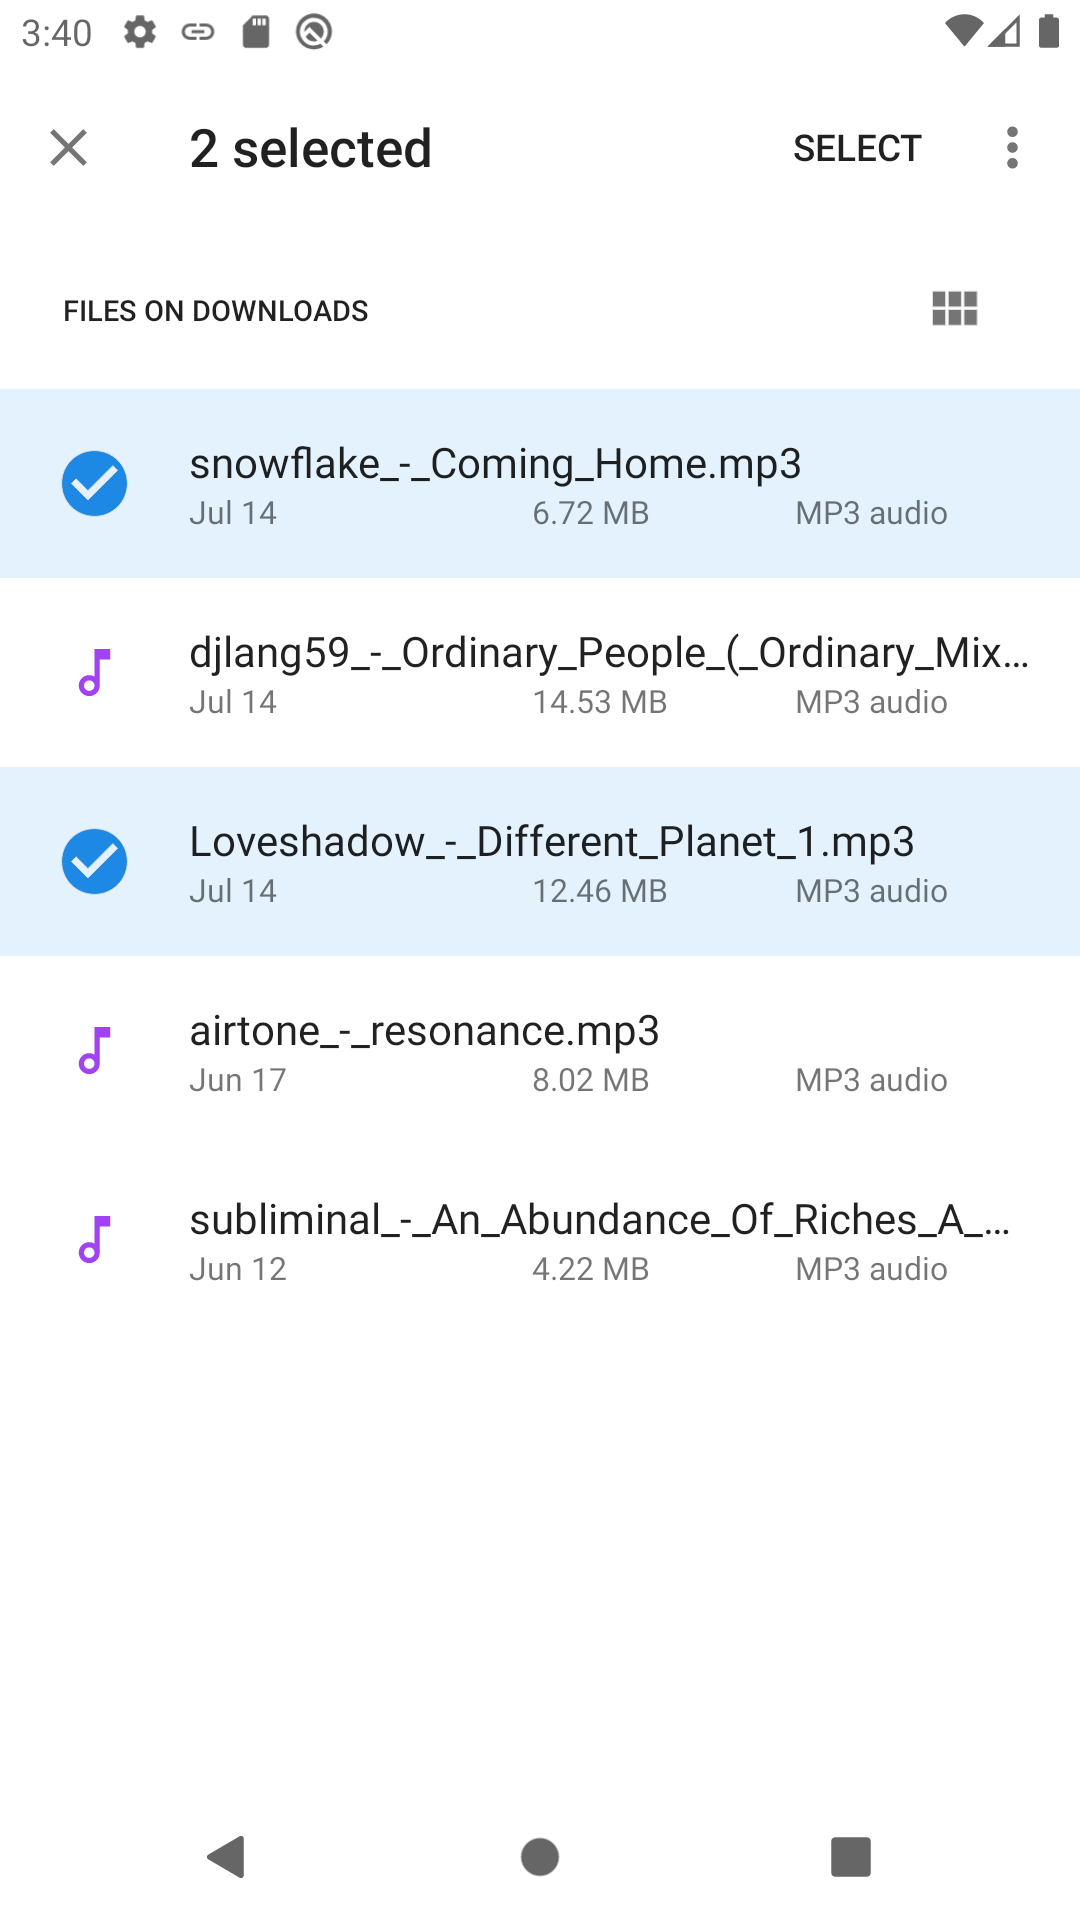
\includegraphics[width=0.3\textwidth]{implementation/screenshot-submit-release.png}
    \caption{Dialog for creating and publishing a new Release}
    \label{fig:submit-release-dialog}
\end{figure}
\begin{figure}
    \centering
    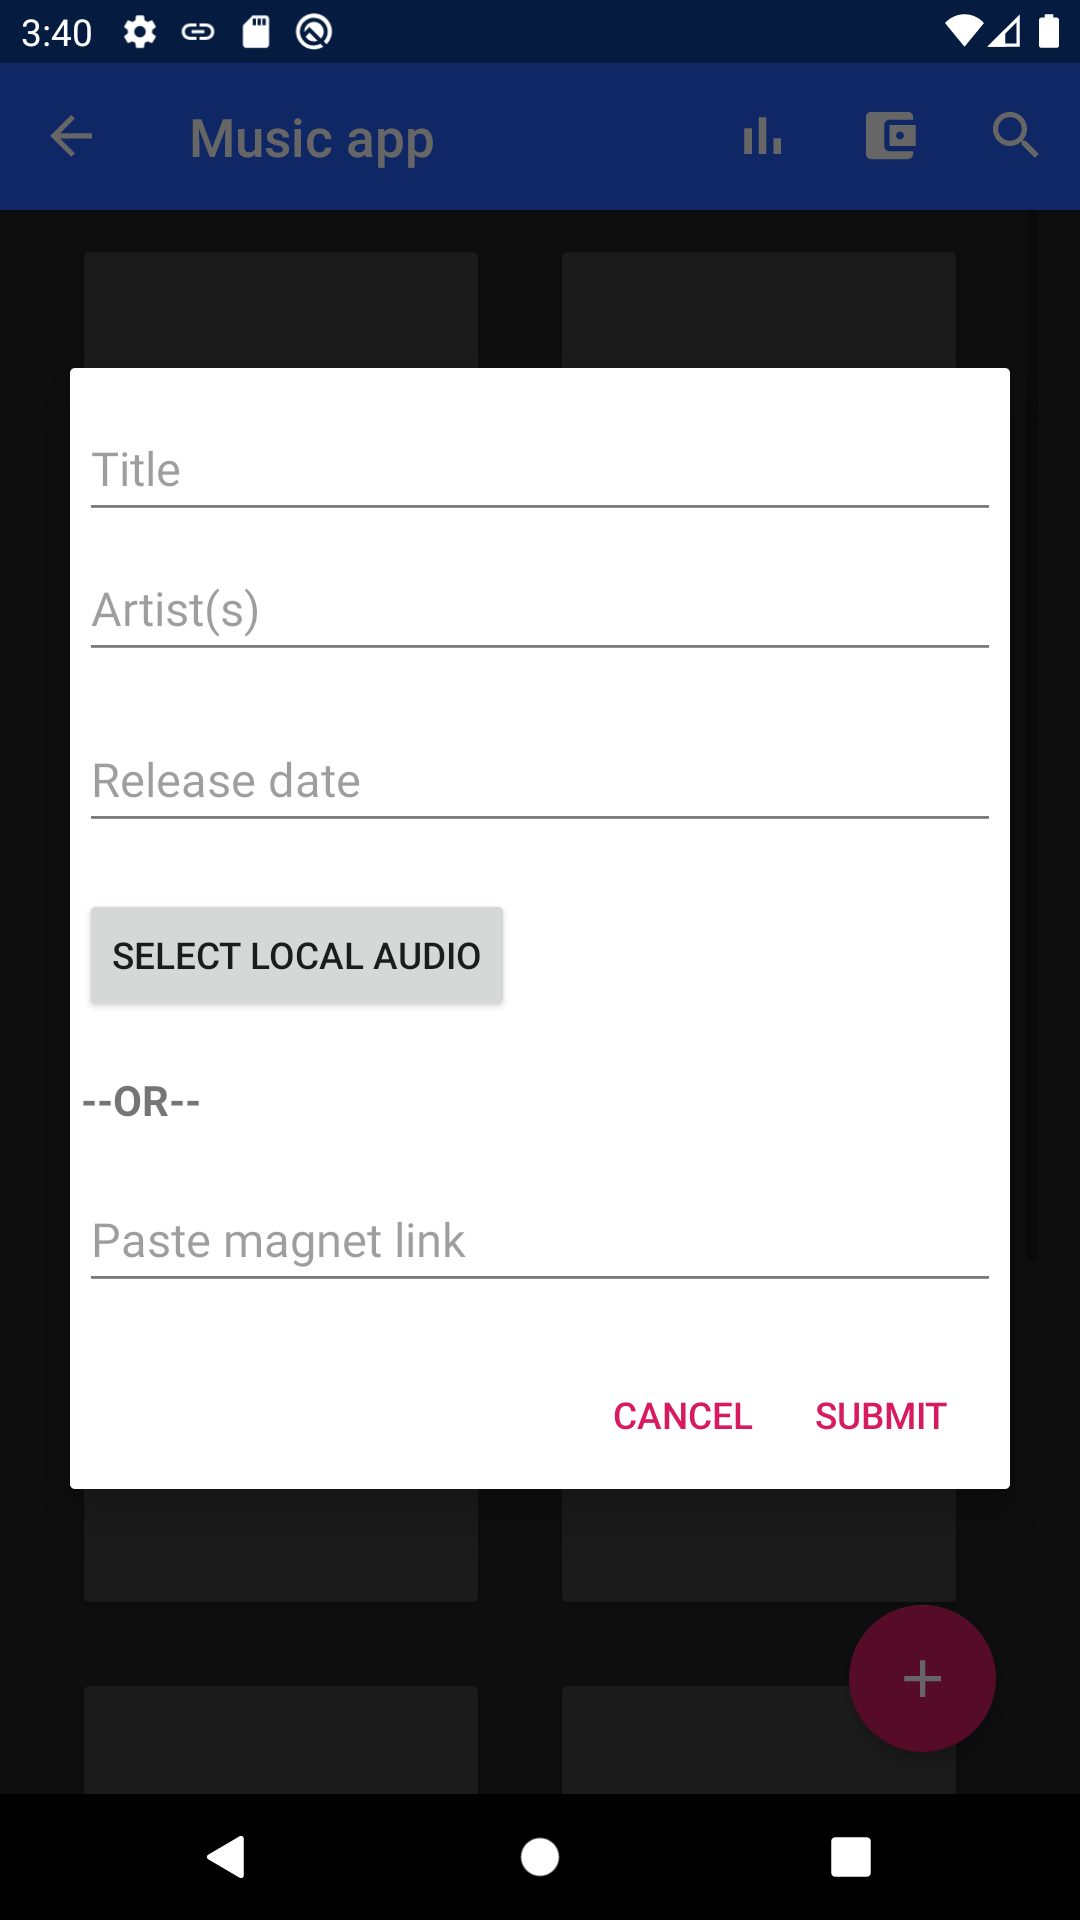
\includegraphics[width=0.3\textwidth]{implementation/screenshot-select-tracks.png}
    \caption{Selecting local tracks for creating a new Release}
    \label{fig:select-tracks}
\end{figure}
\begin{figure}
    \centering
    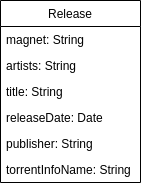
\includegraphics[width=0.3\textwidth]{implementation/release-implementation.png}
    \caption{Release blocks structure as seen on TrustChain}
    \label{fig:release-implementation}
\end{figure}
\begin{figure}
    \centering
    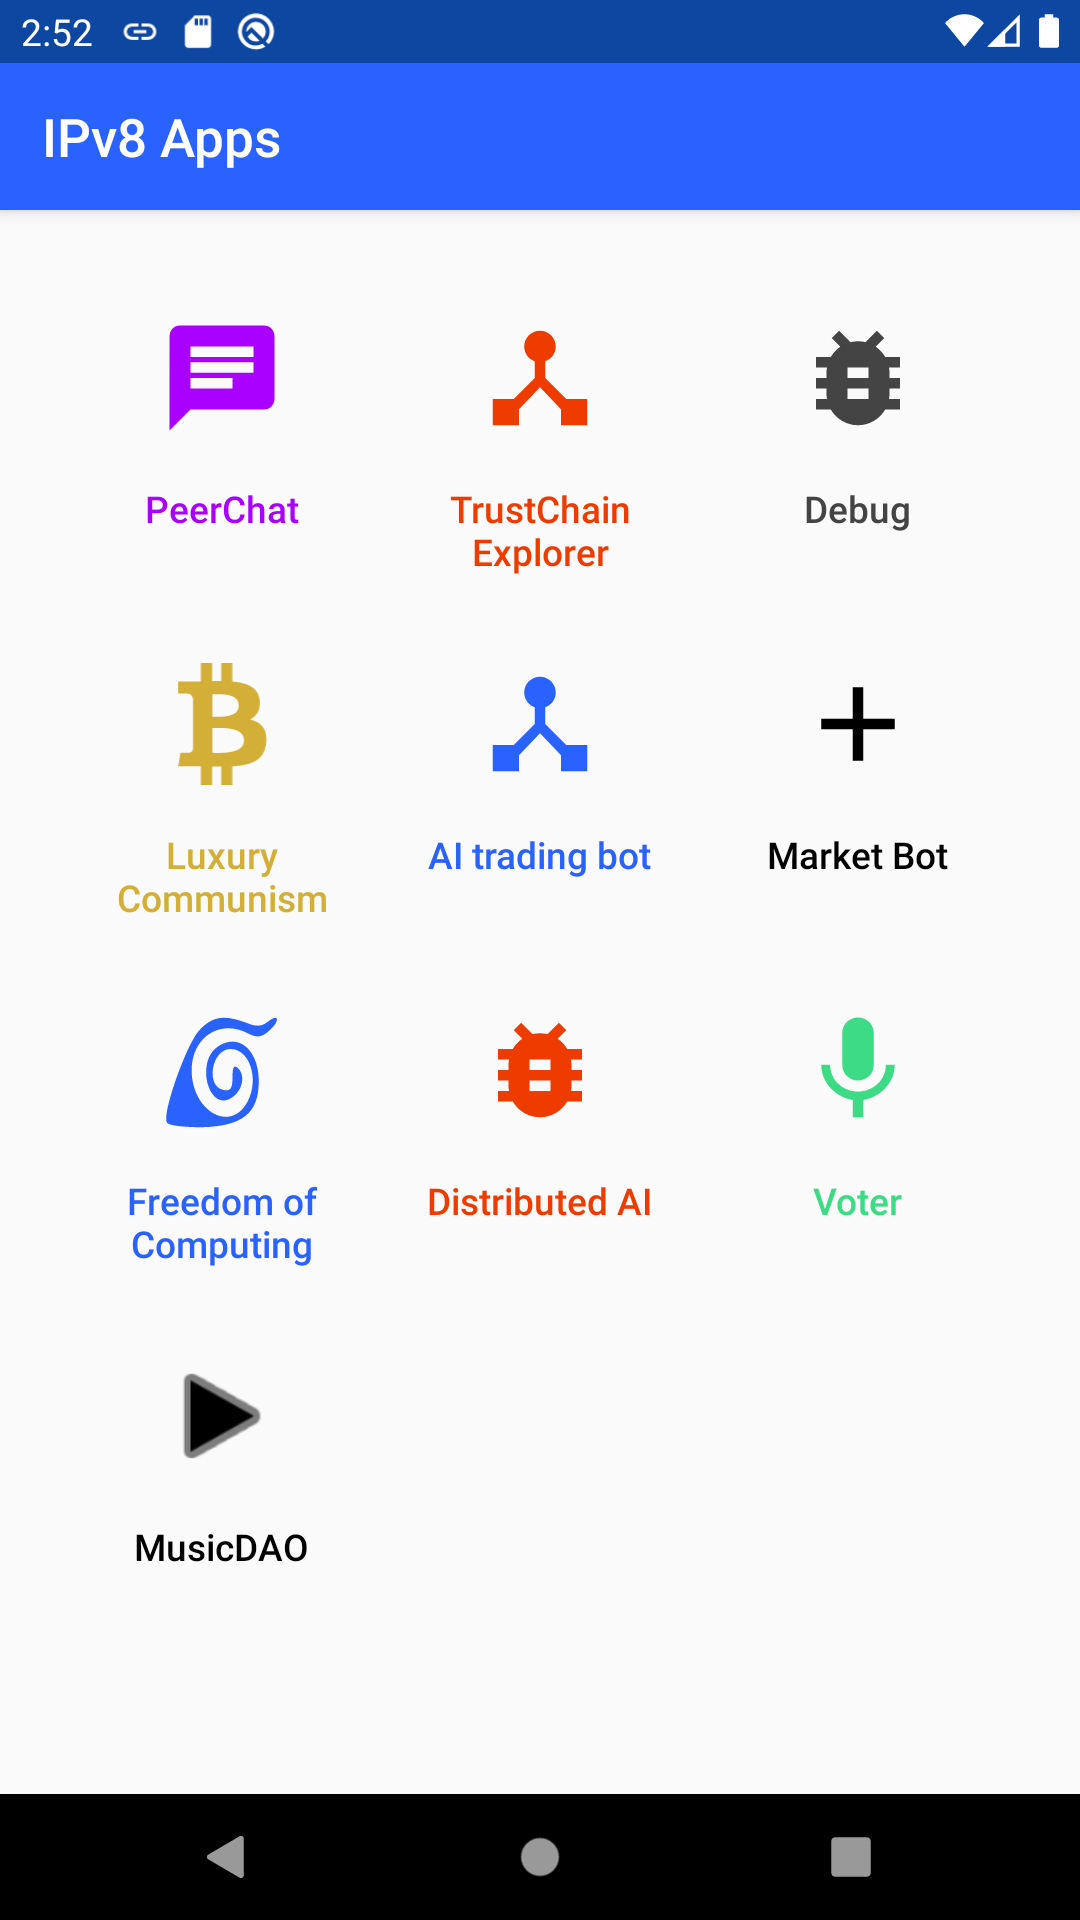
\includegraphics[width=0.3\textwidth]{implementation/screenshot-superapp.png}
    \caption{The app is integrated as a mini-app in the IPv8 Superapp catalog}
    \label{fig:screenshot-superapp}
\end{figure}
\section{Playlist overview}
The playlist overview screen, as shown in \ref{fig:screenshot-home} is the screen that is first shown upon starting the MusicDAO. Here the user is presented a list of playlists, loaded from their local database TrustChain instance. Each Playlists fragment corresponds to one Release block (see ref). In the background runs an iterative process which checks whether new playlist content is found, and re-renders the view if necessary.  re-rendered with the up-to-date list of playlists. The playlists are sorted on their torrent swarm health in ascending order. 
\begin{figure}
    \centering
    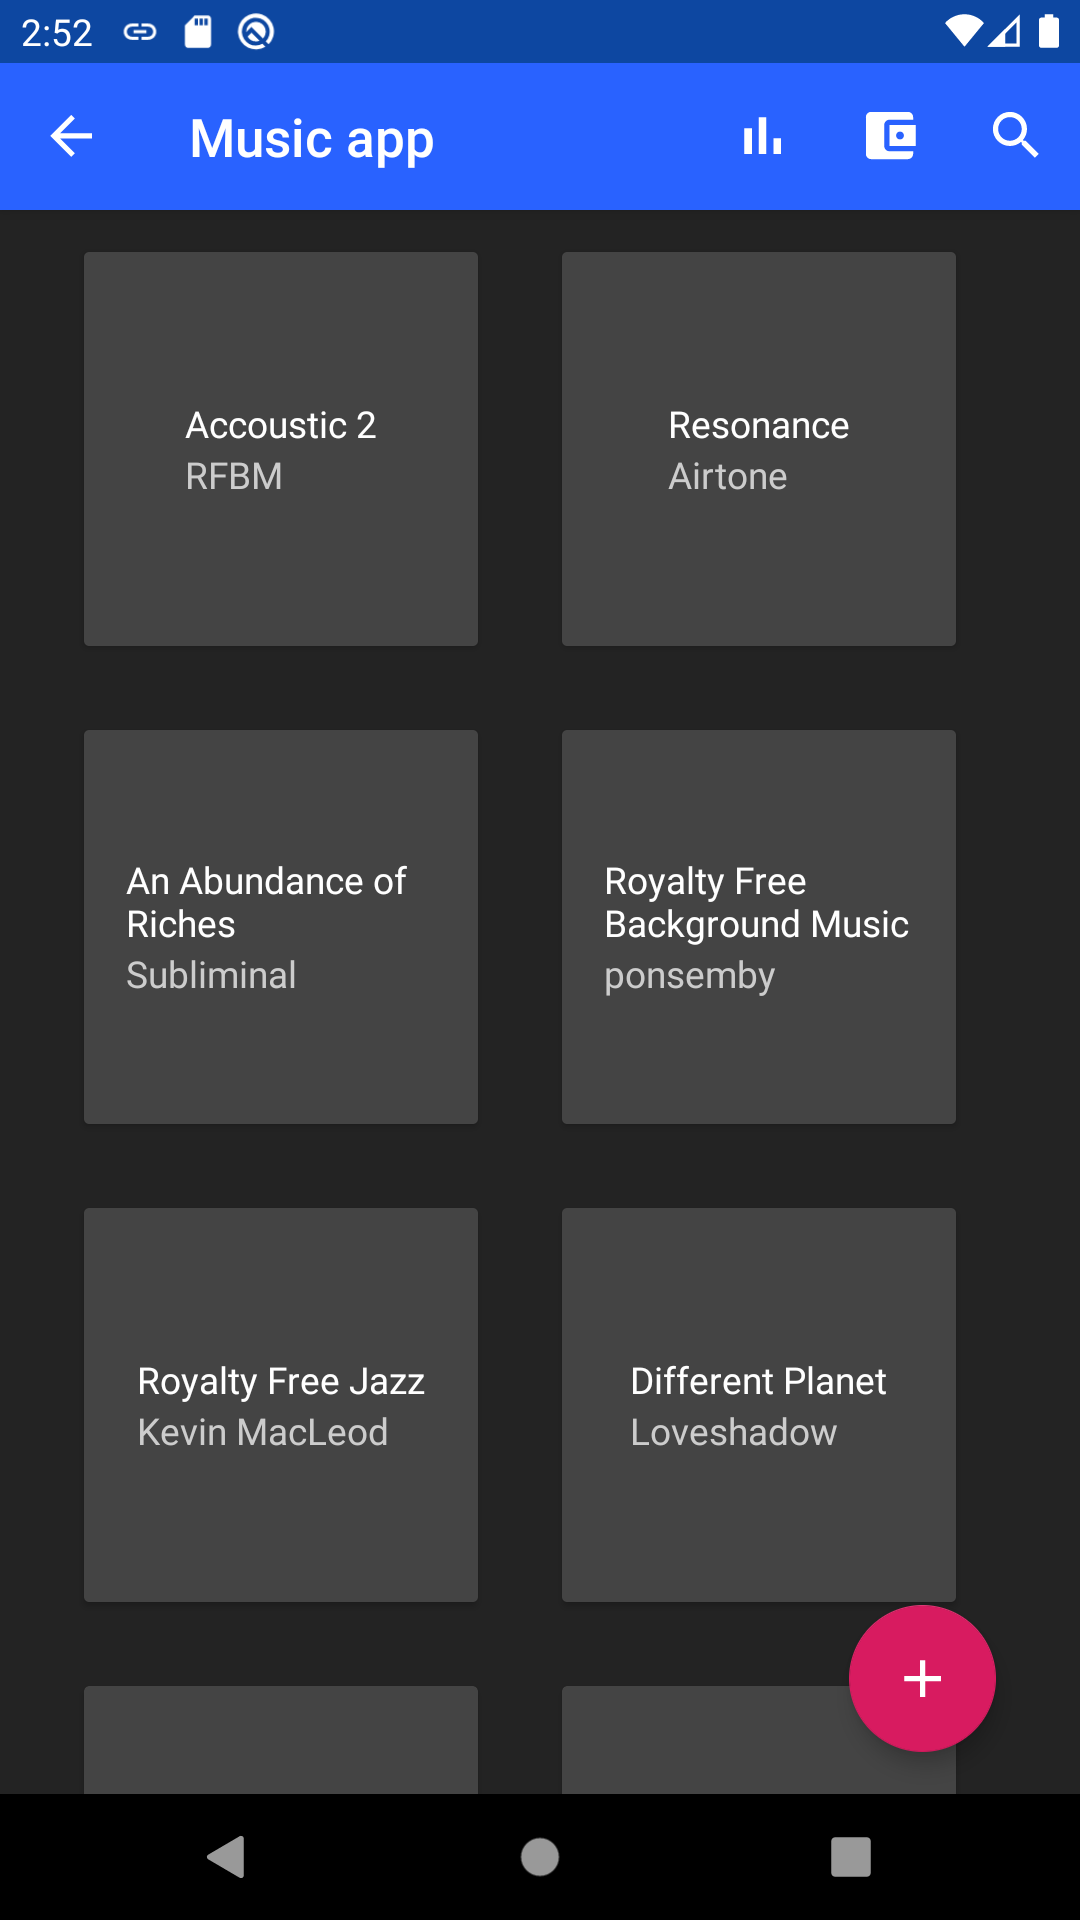
\includegraphics[width=0.3\textwidth]{implementation/screenshot-home.png}
    \caption{The playlist overview screen, which is the entrance screen}
    \label{fig:screenshot-home}
\end{figure}
\section{Playlist fragment}
A Playlist fragment interacts with exactly one Release object. The playlist fragment displays its list of tracks and other metadata, such as the title and artists of the Release (see \ref{fig:screenshot-playlist}). On the right side of each track is a loading indicator, which shows, in real-time how much of the track is downloaded.
\begin{figure}
    \centering
    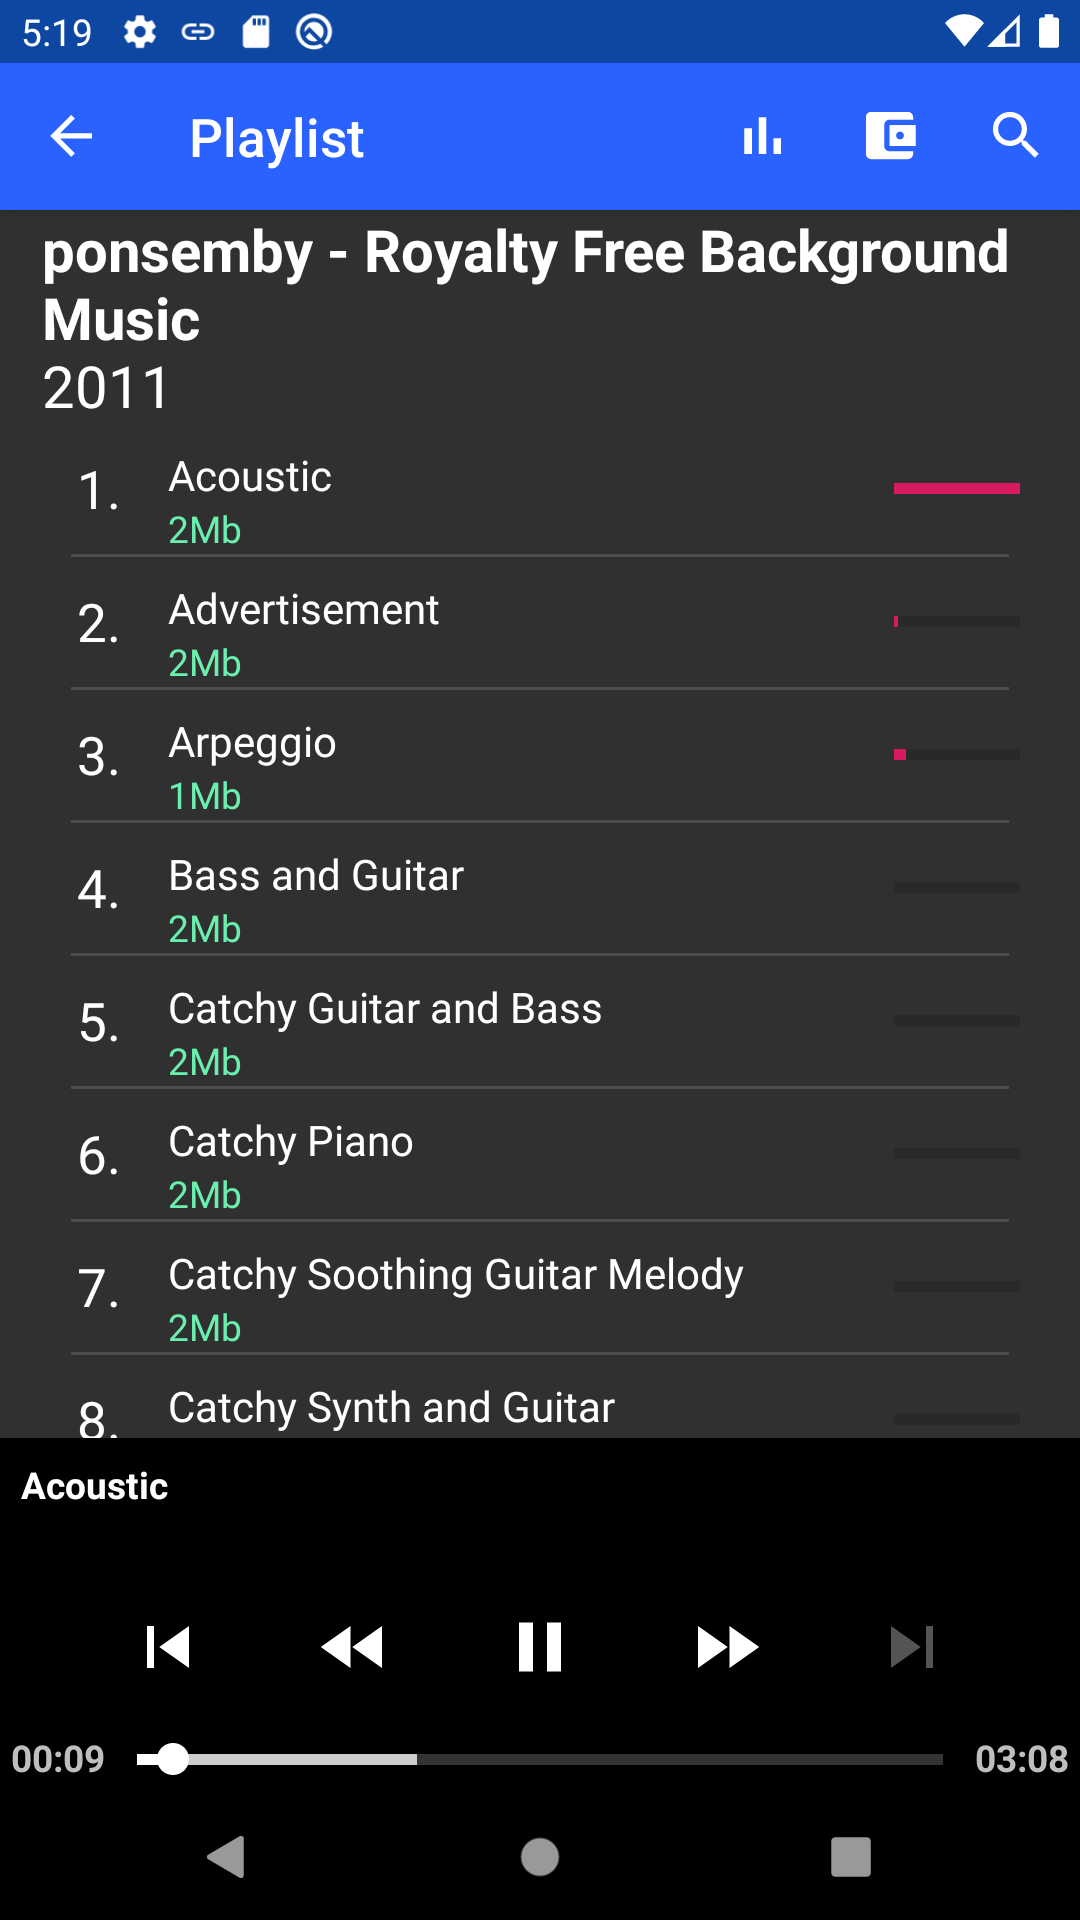
\includegraphics[width=0.3\textwidth]{implementation/screenshot-playlist.png}
    \caption{Playlist fragment}
    \label{fig:screenshot-playlist}
\end{figure}
\subsection{Priority handling}
To provide the user with selected content as soon as possible, we implemented a system which sets priorities on certain tracks and torrent chunks. This uses the piece priorities system in libtorrent, which range from the integers 1 (normal) to 7 (highest) (see libtorrent Manual\footnote{\url{https://www.libtorrent.org/manual-ref.html\#file-format}}). When a user selects a track, this track is given a high \textit{file\_priority} of 5. This is a higher priority than that of other files, so JLibtorrent asks actively for peers who have this file. In addition, the first 5  pieces of the selected track are given a \textit{piece\_priority} of 7, so that the first seconds of the track are buffered quickly and the user can start streaming early.
\subsection{Seeking and buffering}
The music player tries to play the track once a satisfactory portion is loaded. This is implemented as follows. Upon seeking a part of the track, the torrent piece index on which the cursor is located is calculated. Afterwards, the piece at this index and the 5 consequent pieces are given a \textbf{piece\_priority} of 7, which is higher than the other pieces. Once at least 2000 ms from the cursor is buffered, the music player starts playing the track. This way the user can start playing the portion of the track they are most interested in quickly.
